\documentclass[a4 paper]{article}
\usepackage[inner=2.0cm,outer=2.0cm,top=2.5cm,bottom=2.5cm]{geometry}
\usepackage{setspace}
\usepackage[ruled]{algorithm2e}
\usepackage[rgb]{xcolor}
\usepackage{verbatim}
\usepackage{subcaption}
\usepackage{amsgen,amsmath,amstext,amsbsy,amsopn,tikz,amssymb,tkz-linknodes}
\usepackage{fancyhdr}
\usepackage[colorlinks=true, urlcolor=blue,  linkcolor=blue, citecolor=blue]{hyperref}
\usepackage[colorinlistoftodos]{todonotes}
\usepackage{rotating}
\usepackage{booktabs}
\newcommand{\ra}[1]{\renewcommand{\arraystretch}{#1}}

\newtheorem{thm}{Theorem}[section]
\newtheorem{prop}[thm]{Proposition}
\newtheorem{lem}[thm]{Lemma}
\newtheorem{cor}[thm]{Corollary}
\newtheorem{defn}[thm]{Definition}
\newtheorem{rem}[thm]{Remark}

\newcommand{\homework}[6]{
   \pagestyle{myheadings}
   \thispagestyle{plain}
   \newpage
   \setcounter{page}{1}
   \noindent
   \begin{center}
   \framebox{
      \vbox{\vspace{2mm}
    \hbox to 6.28in { {\bf CSE 211:~Discrete Mathematics \hfill {\small (#2)}} }
       \vspace{6mm}
       \hbox to 6.28in { {\Large \hfill #1  \hfill} }
       \vspace{6mm}
       \hbox to 6.28in { {\it Instructor: {\rm #3} \hfill Name: {\rm #5} \hfill Student Id: {\rm #6}} \hfill}
       \hbox to 6.28in { {\it Assistants: #4  \hfill #6}}
      \vspace{2mm}}
   }
   \end{center}
   \markboth{#5 -- #1}{#5 -- #1}
   \vspace*{4mm}
}

\newcommand{\problem}[2]{~\\\fbox{\textbf{Problem #1}}\hfill (#2 points)\newline\newline}
\newcommand{\subproblem}[1]{~\newline\textbf{(#1)}}
\newcommand{\D}{\mathcal{D}}
\newcommand{\Hy}{\mathcal{H}}
\newcommand{\VS}{\textrm{VS}}
\newcommand{\solution}{~\newline\textbf{\textit{(Solution)}} }
\newcommand{\solutionx}{~\textbf{\textit{(Solution)}} }

\newcommand{\bbF}{\mathbb{F}}
\newcommand{\bbX}{\mathbb{X}}
\newcommand{\bI}{\mathbf{I}}
\newcommand{\bX}{\mathbf{X}}
\newcommand{\bY}{\mathbf{Y}}
\newcommand{\bepsilon}{\boldsymbol{\epsilon}}
\newcommand{\balpha}{\boldsymbol{\alpha}}
\newcommand{\bbeta}{\boldsymbol{\beta}}
\newcommand{\0}{\mathbf{0}}


\begin{document}
\homework{Homework \#3}{Due: 15/12/19}{Dr. Zafeirakis Zafeirakopoulos}{Gizem S\"ung\"u, Başak Karakaş}{}{}
\textbf{Course Policy}: Read all the instructions below carefully before you start working on the assignment, and before you make a submission.
\begin{itemize}
\item It is not a group homework. Do not share your answers to anyone in any circumstance. Any cheating means at least -100 for both sides. 
\item Do not take any information from Internet.
\item No late homework will be accepted. 
\item For any questions about the homework, send an email to gizemsungu@gtu.edu.tr
\item Submit your homework into Assignments/Homework3 directory of the CoCalc project CSE211-2019-2020.
\end{itemize}

\problem{1: Hamilton Circuits}{10+10+10=30}
Determine whether there is a Hamilton circuit for each given graph (See Figure \ref{fig:G1a}, Figure \ref{fig:G1b}, Figure \ref{fig:G1c} ). If the graph has a Hamilton circuit, show the path with its vertices which gives a Hamilton circuit. If it does not, explain why no Hamilton circuit exists. \newline
\begin{figure*}[h]
    \centering
    \begin{subfigure}[h]{0.5\textwidth}
        \centering
        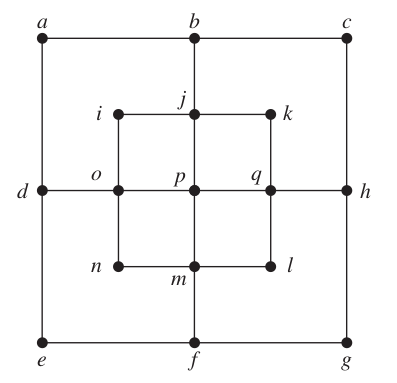
\includegraphics[height=1.5in]{circuit-a.png}
        \caption{The graph $G_1$}
        \label{fig:G1a}
    \end{subfigure}%
    \begin{subfigure}[h]{0.5\textwidth}
        \centering
        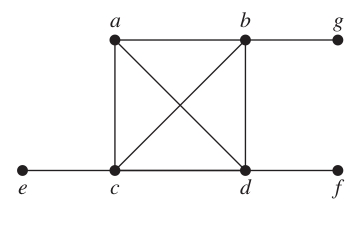
\includegraphics[height=1.5in]{circuit-b.png}
        \caption{The graph $G_2$}
        \label{fig:G1b}
    \end{subfigure}
        \begin{subfigure}[h]{0.5\textwidth}
        \centering
        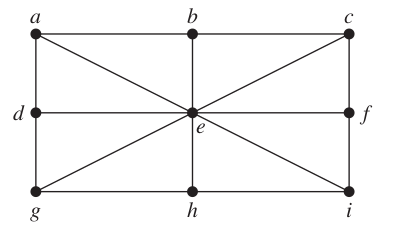
\includegraphics[height=1.2in]{circuit-c.png}
        \caption{The graph $G_3$}
        \label{fig:G1c}
    \end{subfigure}
    \caption{The graphs to find Hamilton circuits for Problem 1}
\end{figure*}

\subproblem{a} \solutionx\\

\subproblem{b} \solutionx\\
\subproblem{c} \solutionx\\

\newpage
\problem{2: Graph Isomorphism}{10+10+10=30}
Determine whether each pair of graphs (see Figure \ref{fig:G2a}, Figure \ref{fig:G2b}, Figure \ref{fig:G2c}) is isomorphic or not.\\
$\textit{Note: If you answer only "isomorphic" or "not isomorphic", you cannot get points. Show your work.}$\\
\begin{figure*}[h]
    \centering
    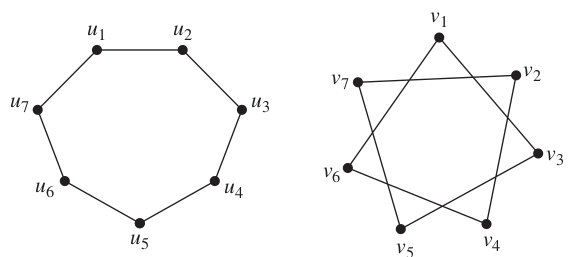
\includegraphics[height=1.7in]{iso-a.png}
    \caption{The graphs $G_{a1}$(left) and $G_{a2}$(right) to find isomorphism for Problem 2(a)}
    \label{fig:G2a}
\end{figure*}

\begin{figure*}[h]
    \centering
    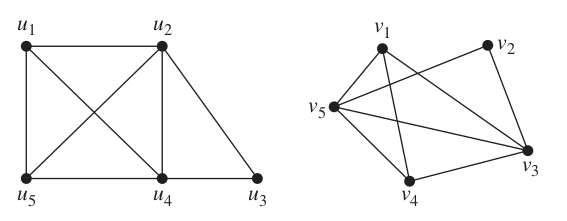
\includegraphics[height=1.5in]{iso-b.png}
    \caption{The graphs $G_{b1}$(left) and $G_{b2}$(right) to find isomorphism for Problem 2(b)}
    \label{fig:G2b}
\end{figure*}

\begin{figure*}[h]
    \centering
    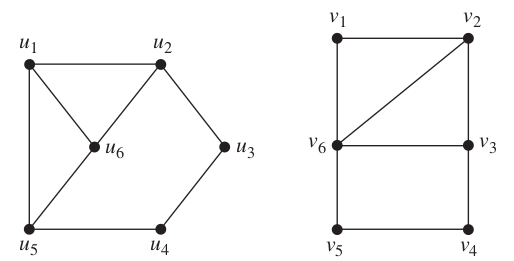
\includegraphics[height=1.5in]{iso-c.png}
    \caption{The graphs $G_{c1}$(left) and $G_{c2}$(right) to find isomorphism for Problem 2(c)}
    \label{fig:G2c}
\end{figure*}

\subproblem{a}\solutionx\\
\subproblem{b}\solutionx\\
\subproblem{c}\solutionx\\
\newpage
\problem{3: Euler Circuits }{10+10=20}
Determine whether there is a Euler circuit for each given graph (See Figure \ref{fig:G3a}, Figure \ref{fig:G3b}). If the graph has a Euler circuit, show the path with its vertices which gives a Euler circuit. If it does not, explain why no Euler circuit exists. \newline

\begin{figure*}[h]
    \centering
    \begin{subfigure}[h]{0.5\textwidth}
        \centering
        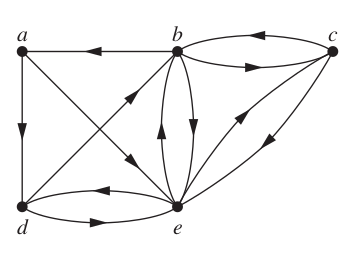
\includegraphics[height=1.5in]{euler-a.png}
        \caption{The graph $G_{3a}$}
        \label{fig:G3a}
    \end{subfigure}%
    \begin{subfigure}[h]{0.5\textwidth}
        \centering
        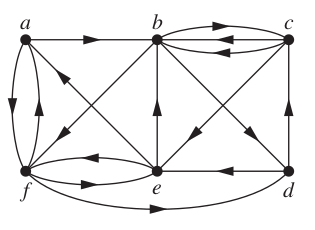
\includegraphics[height=1.5in]{euler-b.png}
        \caption{The graph $G_{3b}$}
        \label{fig:G3b}
    \end{subfigure}
    \caption{The graphs to find Euler circuits for Problem 3}
\end{figure*}

\solution
\newline
\newline
\newline
\newline
\newline
\newline
\problem{4: Applications on Graphs}{20}
Schedule the final exams for Math 101, Math 243, CSE 333, CSE 346, CSE 101, CSE 102, CSE 273, and CSE 211, using the fewest number of different time slots, if there are no students who are taking:
\begin{itemize}
    \item both Math 101 and CS 211,
    \item both Math 243 and CS 211,
    \item both CSE 346 and CSE 101,
    \item both CSE 346 and CSE 102,
    \item both Math 101 and Math 243,
    \item both Math 101 and CSE 333,
    \item both CSE 333 and CSE 346
\end{itemize}
but there are students in every other pair of courses together for this semester.\\ 
$\textbf{Note:}$ Assume that you have only one classroom.\\ \\
$\textit{Hint 1: Solve the problem with respect to your problem session notes.}$\\
$\textit{Hint 2: \hyperlink{https://www.draw.io/}{Check the website}}$
\newline
\solution
\end{document} 


